\section{Introducción}
Un \textbf{octree} es una estructura de datos en la cual cada nodo tiene exactamente ochos hijos. Como muestra la figura \ref{fig:octree}, este se subdivide recursivamente en octantes.\cite{wiki:octree}
\begin{figure}[H]
  \centering
  \fbox{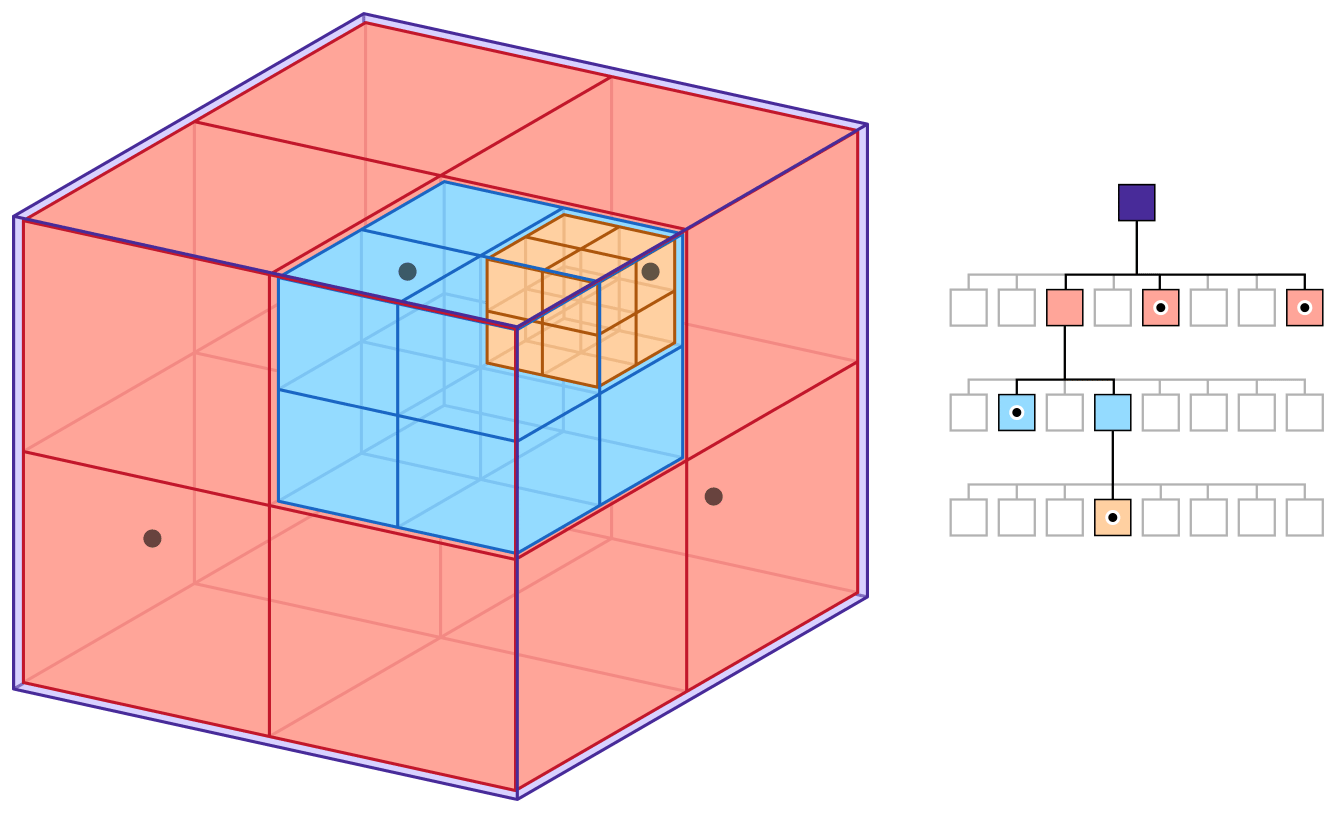
\includegraphics[width=0.8\textwidth]{octree}}
  \caption{Un cubo se subdivide recursivamente en ocho octantes, formando así la estructura de un árbol.}
  \label{fig:octree}
\end{figure}

\subsection{Usos comunes}
A menudo usamos octrees en:
\begin{itemize}
    \item Renderizado en gráficos 3D.
    \item El problema de \textit{Nearest neighborhod}.
    \item Análisis finito de elementos.
    \item \textit{Sparse voxel octree}.
    \item Grillas no estructuradas.
\end{itemize}